\documentclass[11pt,a4paper]{article}

\usepackage[spanish]{babel}
\usepackage[utf8]{inputenc}
\usepackage{amsmath, amssymb}
\usepackage{graphicx}
\usepackage{float}
\usepackage{geometry}
\usepackage{booktabs}
\usepackage{physics}
\usepackage{siunitx}
\usepackage{subcaption}
\usepackage{multirow}

\geometry{margin=2.5cm}

\title{Simulación numérica de proyectiles reales:\\
Aplicación al béisbol y al golf}

\author{Andrés López Serna}

\date{\today}

\begin{document}

\maketitle

\begin{abstract}
En este trabajo se estudia numéricamente el movimiento de proyectiles sometidos a fuerzas aerodinámicas utilizando el método de Euler. Se analizan dos sistemas físicos: el bateo en 2D de una pelota de béisbol teniendo en cuenta la fuerza de arrastre y la presencia de viento y el lanzamiento en 3D de una pelota de golf añadiendo el efecto Magnus. Los resultados muestran cómo factores como la rugosidad, el giro y el viento modifican de manera sustancial el alcance, el ángulo óptimo y la desviación lateral del lanzamiento.
\end{abstract}

\section{Introducción}

Los lanzamientos en condiciones reales se alejan de una trayectoria parabólica ideal debido a la presencia de fuerzas aerodinámicas. En particular, la resistencia del aire introduce una fuerza no lineal dependiente de la velocidad, mientras que la rotación del proyectil genera una fuerza conocida como efecto Magnus.

En este trabajo se estudian dos aplicaciones deportivas representativas:

\begin{itemize}
\item La dinámica en 2D de una pelota de béisbol bateada considerando, además de la gravedad, la fuerza de arrastre debida a la presencia de aire y el efecto de la presencia de viento lateral.
\item El lanzamiento en 3D de una pelota de golf considerando además los efectos derivados de su rugosidad y espín.
\end{itemize}

Ambos casos permiten analizar cómo diferentes mecanismos aerodinámicos alteran el alcance y la trayectoria respecto al modelo ideal.

\section{Marco Teórico General}
El marco teórico se desarrolla a partir de la segunda ley de Newton, utilizando como apoyo el libro \textit{Computational Physics} de  N. J. Giordano y H. Nakanishi \cite{giordano}. De esta forma, se obtendrán las ecuaciones diferenciales resolubles mediante integración numérica:

\begin{equation}
m \dv{\vec{v}}{t} = \sum \vec{F}.
\end{equation}

Las primera fuerza considerada es la gravitatoria cuya expresión viene dada por $\vec{F_g}=m\vec{g}$. En ambos modelos se incluye una corrección debida a la altura del objeto (h),aunque su efecto es despreciable en las escalas consideradas durante las simulaciones. Por tanto, la aceleración gravitatoria empleada es:

\begin{equation}
g_{\text{eff}} = g \cdot \left( \frac{R_T}{R_T + h} \right)^2
\end{equation}

Por otro lado, se tiene en cuenta el efecto de la fuerza de arrastre del aire que se define como:

\begin{equation}
\vec{F}_D = -\frac{1}{2}\cdot C_D \cdot \rho \cdot A\cdot  v \cdot \vec{v}.
\end{equation}

En el caso del estudio de una pelota de béisbol se utiliza una dependencia empírica para obtener la aceleración debida al drag:
\[
B_2 = \frac{1}{2m} \cdot C_D \cdot  \rho\cdot  A = 0.0039 + \frac{0.0058}{1 + \exp\left(\frac{v - v_d}{\delta}\right)}.
\]
No obstante, en el caso del golf, para una pelota rugosa, se modeliza la fuerza de arrastre mediante la constante de arrastre:
\[
C_D(v) =
\begin{cases}
1, & \text{si } v > 14, \\
\dfrac{14}{v}, & \text{si } v \le 14
\end{cases}
\Longleftrightarrow C_D(v) = \frac{14}{\max(14,\, v)}.
\]
Mientras tanto, al estudiar el caso de una pelota lisa, se considera que $C_D=1$.

Por último, cuando el proyectil rota con velocidad angular $\vec{\omega}$, aparece una fuerza perpendicular a $\vec{\omega}$ y $\vec{v}$. Por tanto, la fuerza de Magnus es:

\begin{equation}
\vec{F}_M = S_0\cdot \vec{\omega} \times \vec{v}.
\end{equation}

La aceleración asociada es:

\begin{equation}
\vec{a}_M = \frac{S_0}{m} \cdot (\vec{\omega} \times \vec{v}).
\end{equation}

Este término, como se observará en el experimento de la pelota de golf, puede introducir desviaciones laterales en los lanzamientos. 

Finalmente, la aceleración total será la suma de los términos considerados anteriormente:
\begin{equation}
\vec{a}_M = \vec{g_{\text{eff}}}+\vec{a}_D+\vec{a}_M.
\end{equation}

\section{Métodos numéricos}

En ambos casos estudiados, utilizando una función definida por el usuario al comienzo de los archivos .py, las ecuaciones de movimiento se resuelven mediante el método de Euler explícito:

\begin{equation}
\begin{cases}
\vec{r}_{n+1} = \vec{r}_n + \vec{v}_n \,\Delta t \\
\vec{v}_{n+1} = \vec{v}_n + \vec{a}_n \,\Delta t
\end{cases}
\end{equation}
Los pasos temporales utilizados son suficientemente bajos como para poder definir los alcances de los lanzamientos como la media de los dos últimos valores en la dirección x (el último está en $h<0$ y el penúltimo en $h>0$).
\begin{equation}
alcance = (x[-1] + x[-2]) / 2
\end{equation}
También se realiza un barrido angular entre $0^\circ$ y $90^\circ$ para determinar el ángulo que maximice el alcance para el resto de condiciones iniciales.

Por otro lado, en el caso del golf se simulan tres tipos de lanzamientos (Hook, Slice y sin efecto Magnus) para pelota lisa y rugosa y luego se realizará un proceso de optimización para maximizar el alcance del golpe.

\section{Resultados}

En esta sección se presentan los resultados obtenidos para la simulación numérica del bateo de una pelota de béisbol en dos dimensiones y del lanzamiento de una pelota de golf en tres dimensiones incluyendo efecto Magnus.

\subsection{Pelota de béisbol}

Se realizó un barrido angular entre $0^\circ$ y $90^\circ$ con resolución 0.1$^\circ$. Los resultados obtenidos para los modelos con y sin viento se muestran en la Tabla~\ref{tab:beisbol}.

\begin{table}[h]
\centering
\vspace{0.2cm}
\begin{tabular}{lcc}
\hline
Modelo & Alcance máximo (m) & Ángulo óptimo ($^\circ$) \\
\hline
Sin viento & 119.8 & 36.0 \\
Con viento a favor & 135.2 & 38.9 \\
Con viento en contra & 105.0 & 33.6 \\
\hline
\end{tabular}
\caption{Resultados para la pelota de béisbol.}
\label{tab:beisbol}
\end{table}

Se pueden representar los alcances máximos en función del ángulo de lanzamiento (Figura~\ref{fig:beisbol_alcance}) así como las trayectorias optimizadas (Figura~\ref{fig:beisbol_optimizado}).

\begin{figure}[H]
\centering
\begin{subfigure}[t]{0.49\textwidth}
    \centering
    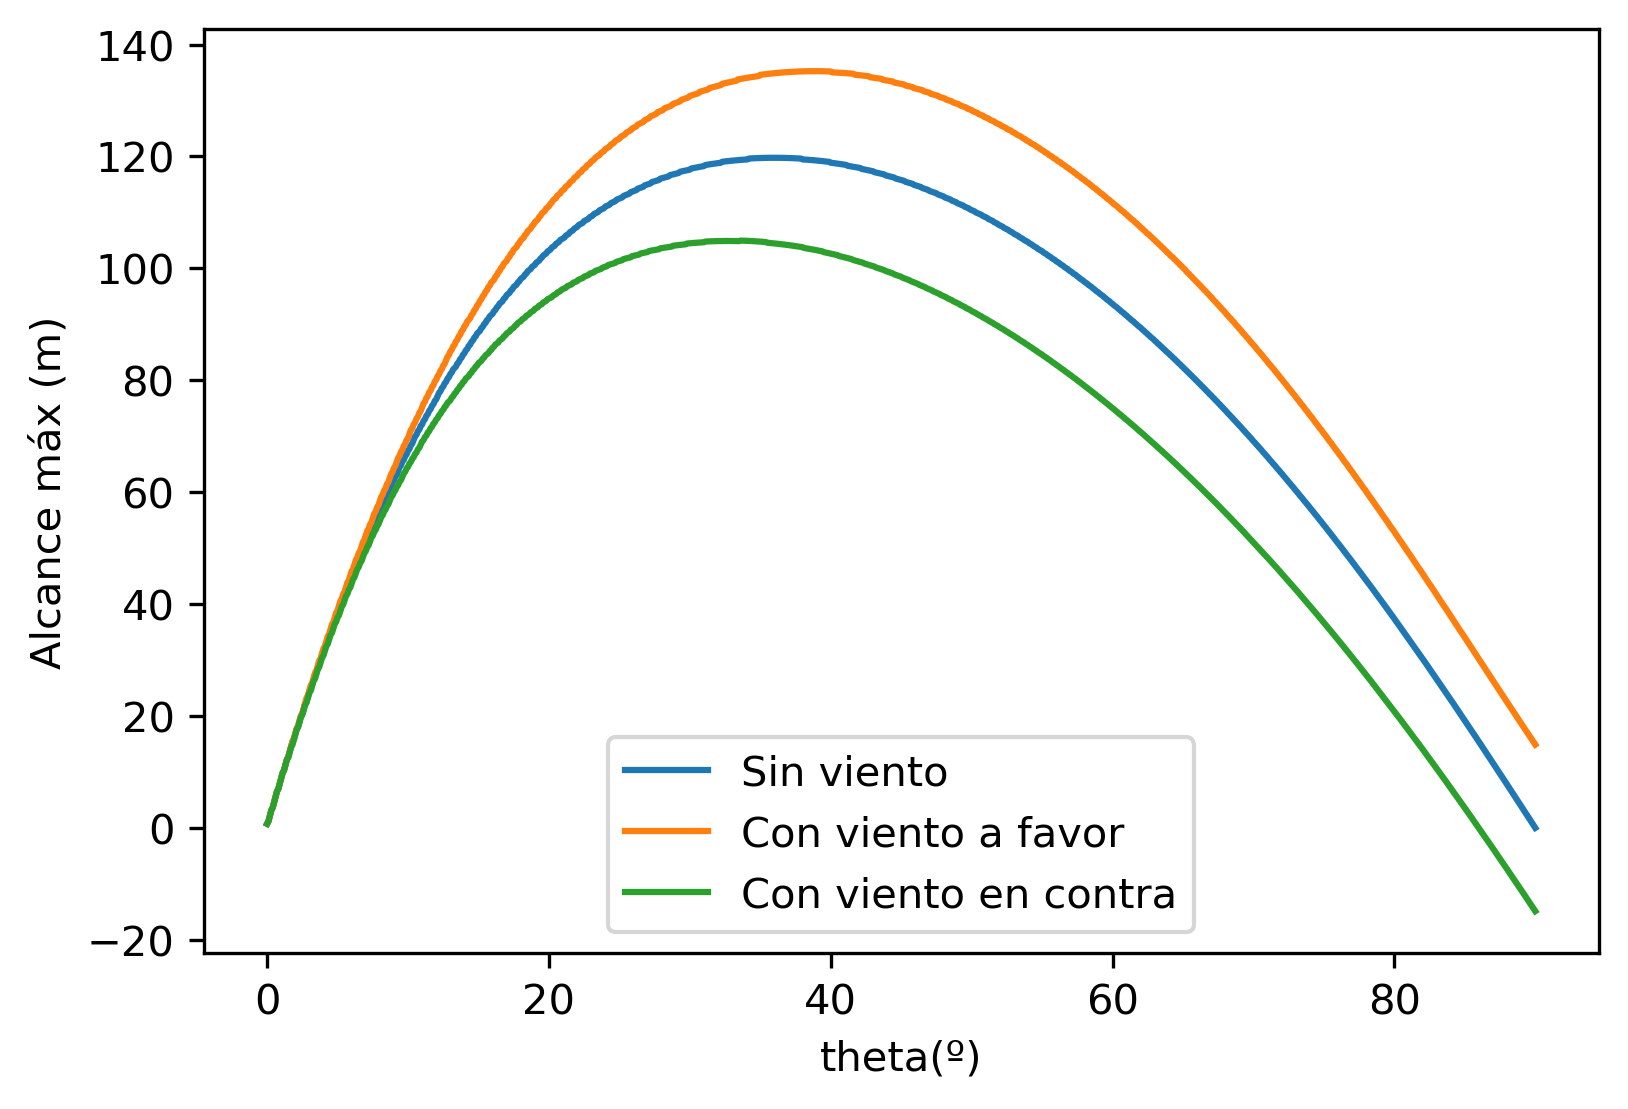
\includegraphics[width=\linewidth]{imagenes/beisbol_alcance.png}
    \caption{Alcance final en función del ángulo inicial.}
    \label{fig:beisbol_alcance}
\end{subfigure}
\hfill
\begin{subfigure}[t]{0.49\textwidth}
    \centering
    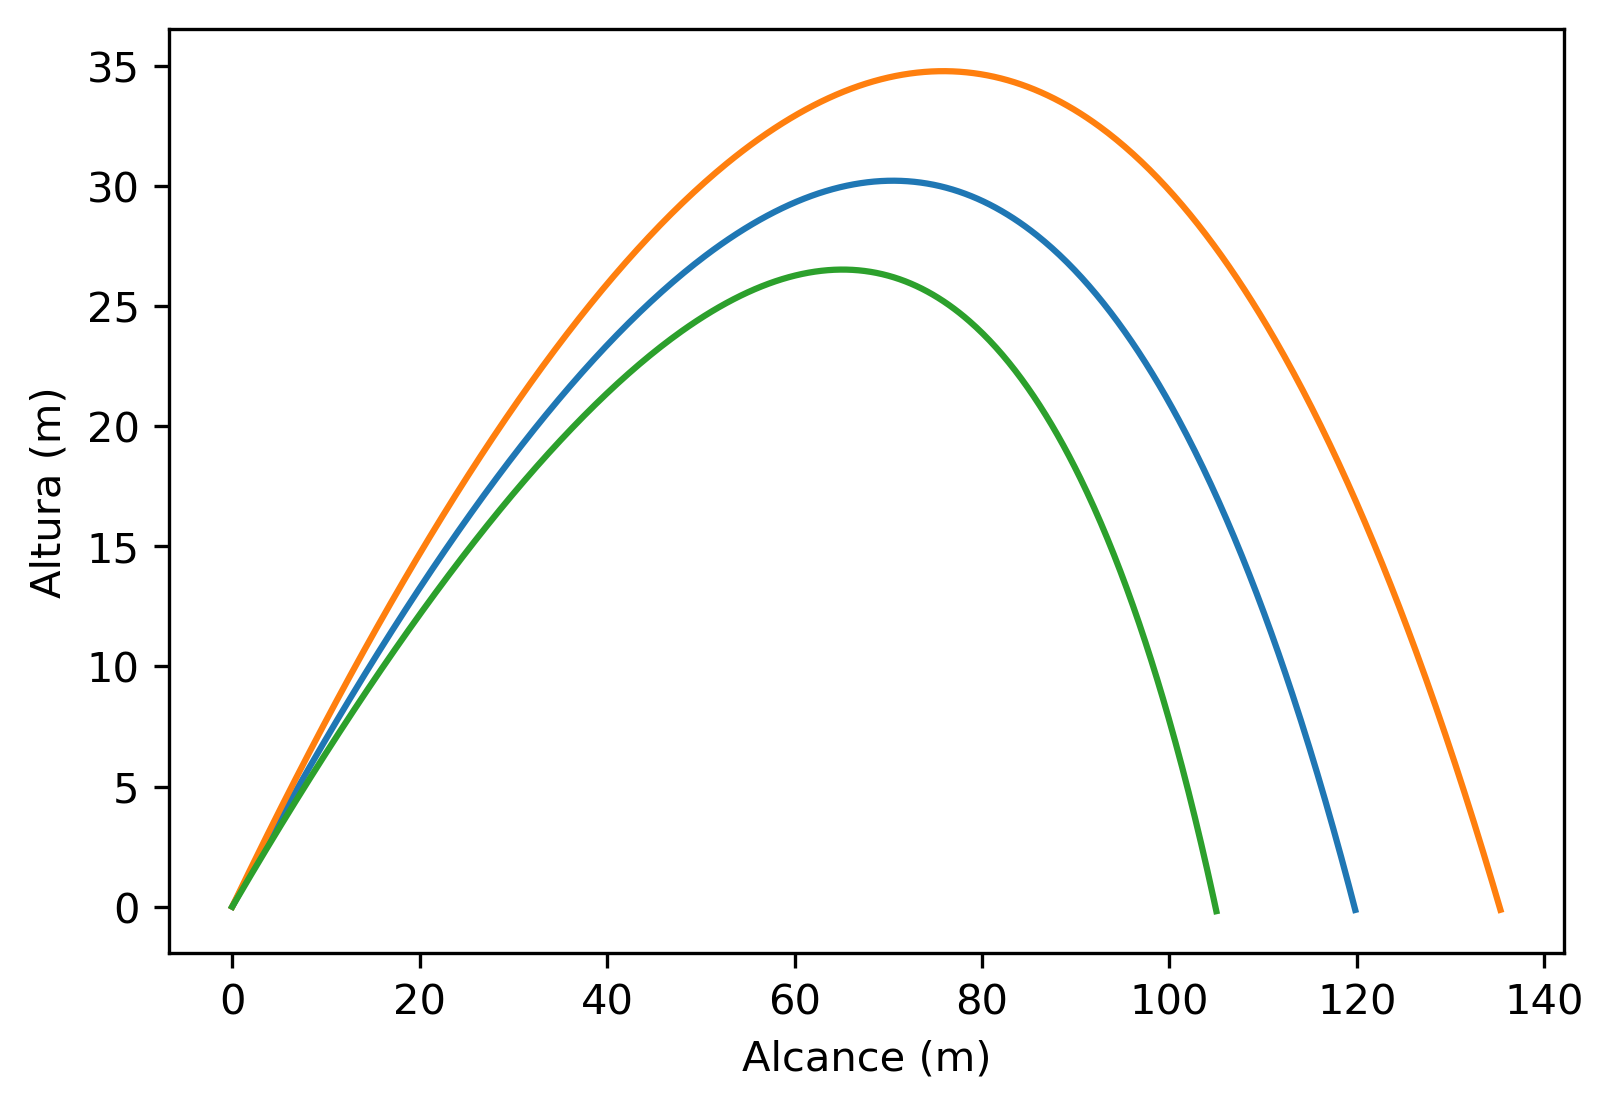
\includegraphics[width=\linewidth]{imagenes/beisbol_optimizado.png}
    \caption{Bateos cuyo alcance está maximizado.}
    \label{fig:beisbol_optimizado}
\end{subfigure}
\caption{Comparación de resultados para la pelota de béisbol.}
\label{fig:beisbol_comparacion}
\end{figure}


\subsection{Pelota de golf}

Se consideraron dos tipos de pelota (rugosa y lisa) y tres tipos de lanzamientos (hook, slice y sin efecto Magnus), además, los casos fueron optimizados en función del ángulo polar inicial; obteniendo los resultados de la tabla~\ref{tab:golf_fijo_sin}, donde se considera el caso sin viento.

\begin{table}[H]
\centering
\begin{tabular}{llccc}
\hline
Tipo de pelota & Configuración & $\theta_{\text{opt}}$ ($^\circ$) & Alcance (m) & Desviación lateral (m) \\
\hline
\multirow{3}{*}{Rugosa} 
& Hook        & 24 & 147.2 & 76.0 \\
& Slice       & 24 & 147.2 & 76.0 \\
& Sin Magnus  & 30 & 180.3 & 0.0 \\
\hline
\multirow{3}{*}{Lisa} 
& Hook        & 28 & 79.0 & 28.7 \\
& Slice       & 28 & 79.0 & 28.7 \\
& Sin Magnus  & 33 & 88.1 & 0.0 \\
\hline
\end{tabular}
\caption{Resultados optimizados para la pelota de golf sin viento.}
\label{tab:golf_fijo_sin}
\end{table}

Además, se optimiza el caso para una velocidad de viento $\vec{v_w}=3\hat{x}+4\hat{y}+5\hat{z}$. (Tabla~\ref{tab:golf_fijo_con})

\begin{table}[H]
\centering
\begin{tabular}{llccc}
\hline
Tipo de pelota & Configuración & $\theta_{\text{opt}}$ ($^\circ$) & Alcance (m) & Desviación lateral (m) \\
\hline
\multirow{3}{*}{Rugosa} 
& Hook        & 23 & 154.2 & 68.2 \\
& Slice       & 24 & 164.9 & 94.5 \\
& Sin Magnus  & 32 & 199.6 & 14.5 \\
\hline
\multirow{3}{*}{Lisa} 
& Hook        & 28 & 93.7 & 21.5 \\
& Slice       & 29 & 98.6 & 50.8 \\
& Sin Magnus  & 35 & 110.6 & 15.9 \\
\hline
\end{tabular}
\caption{Resultados optimizados para la pelota de golf sin viento.}
\label{tab:golf_fijo_con}
\end{table}

Se pueden representar también las trayectorias de los golpes (figura ~\ref{fig:vsgolf})y, además, obtener la vista superior de las trayectorias para analizar la desviación lateral.

\begin{figure}[H]
\centering
\begin{subfigure}[t]{0.49\textwidth}
    \centering
    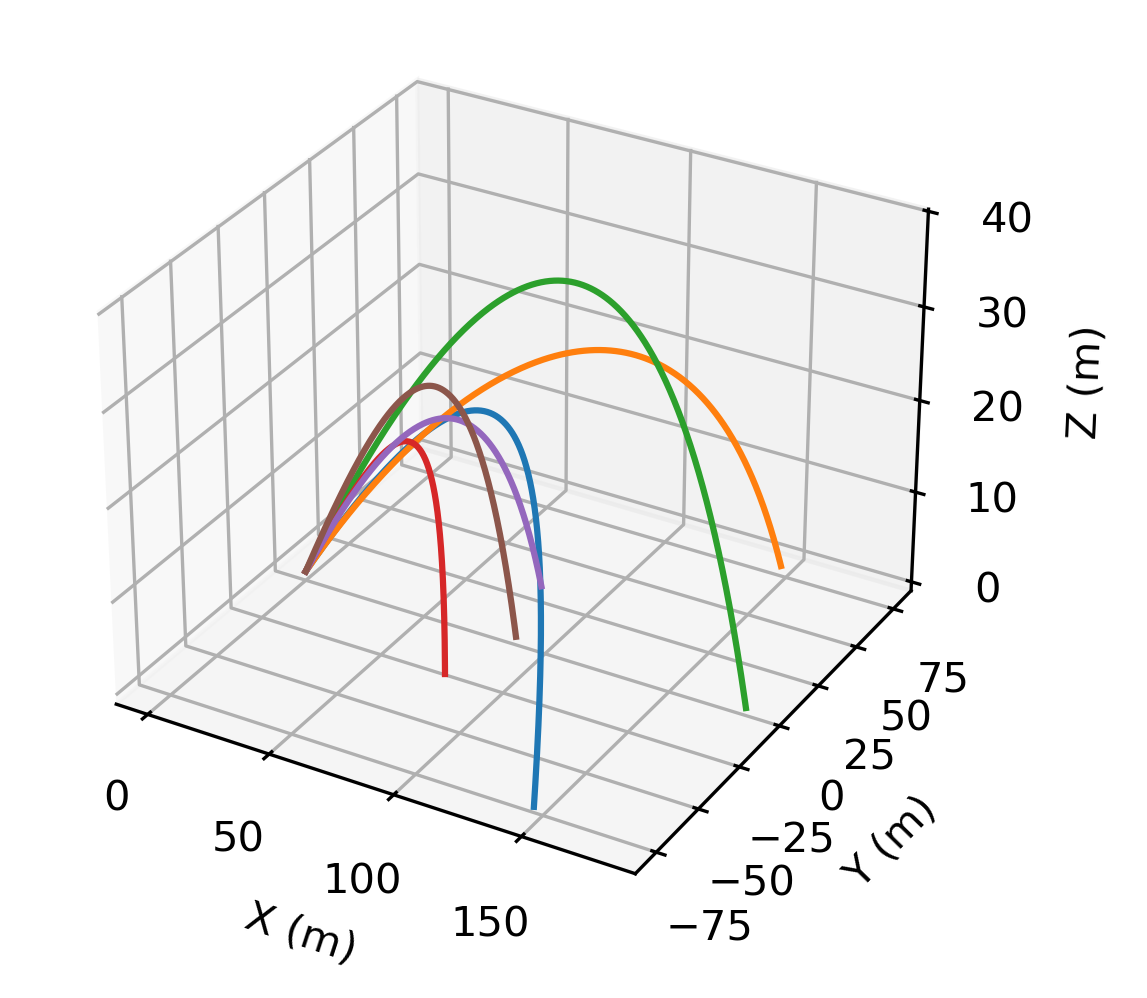
\includegraphics[width=\linewidth]{imagenes/golf_vssin.png}
    \caption{Caso sin viento.}
    \label{fig:vssin}
\end{subfigure}
\hfill
\begin{subfigure}[t]{0.47\textwidth}
    \centering
    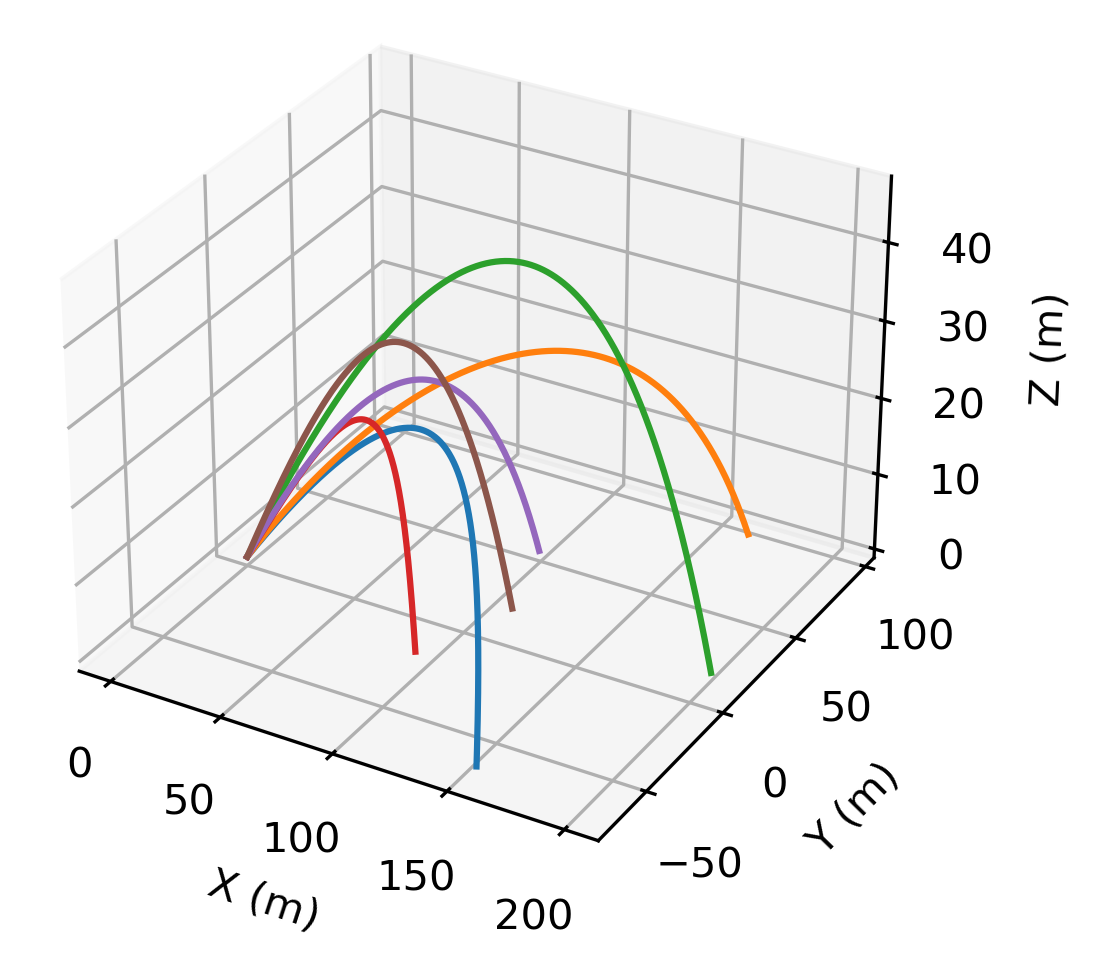
\includegraphics[width=\linewidth]{imagenes/golf_vscon.png}
    \caption{Caso con viento.}
    \label{fig:vscom}
\end{subfigure}
\caption{Trayectorias tridimensionales para una pelota de golf.}
\label{fig:vsgolf}
\end{figure}

\begin{figure}[H]
\centering
\begin{subfigure}[t]{0.49\textwidth}
    \centering
    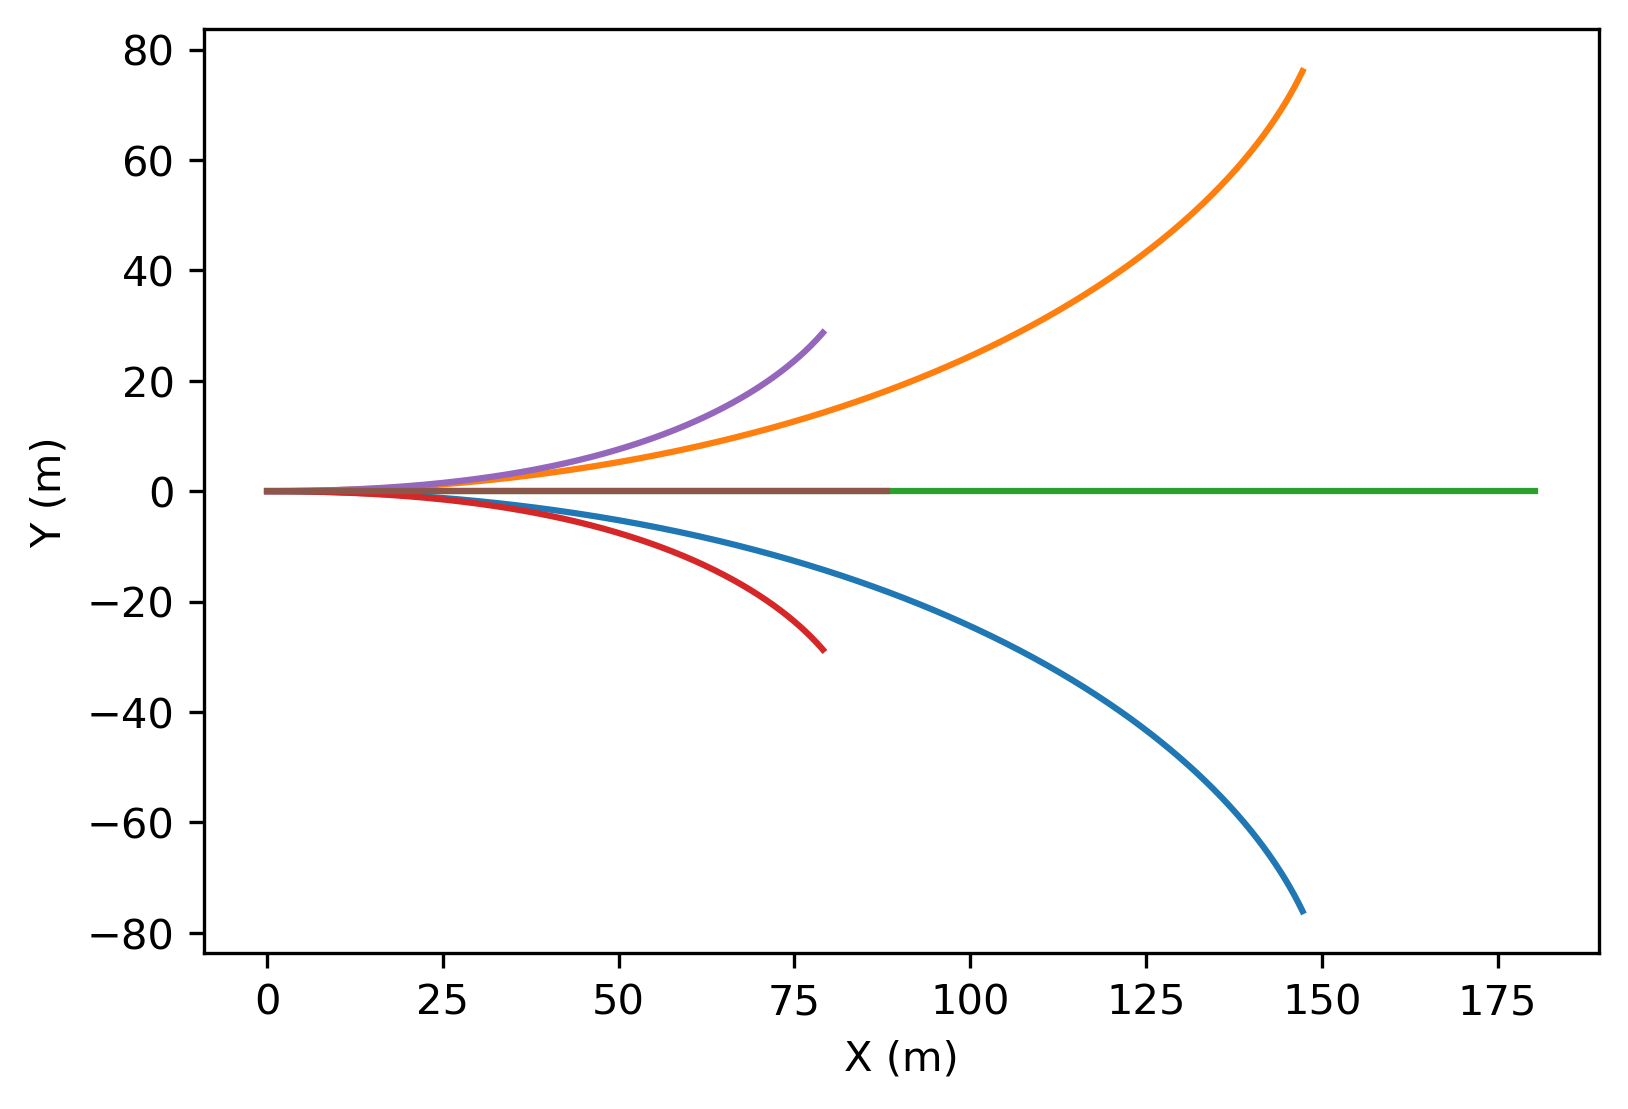
\includegraphics[width=\linewidth]{imagenes/golf_lateralXYsin.png}
    \caption{Caso sin viento.}
    \label{fig:XYsin}
\end{subfigure}
\hfill
\begin{subfigure}[t]{0.49\textwidth}
    \centering
    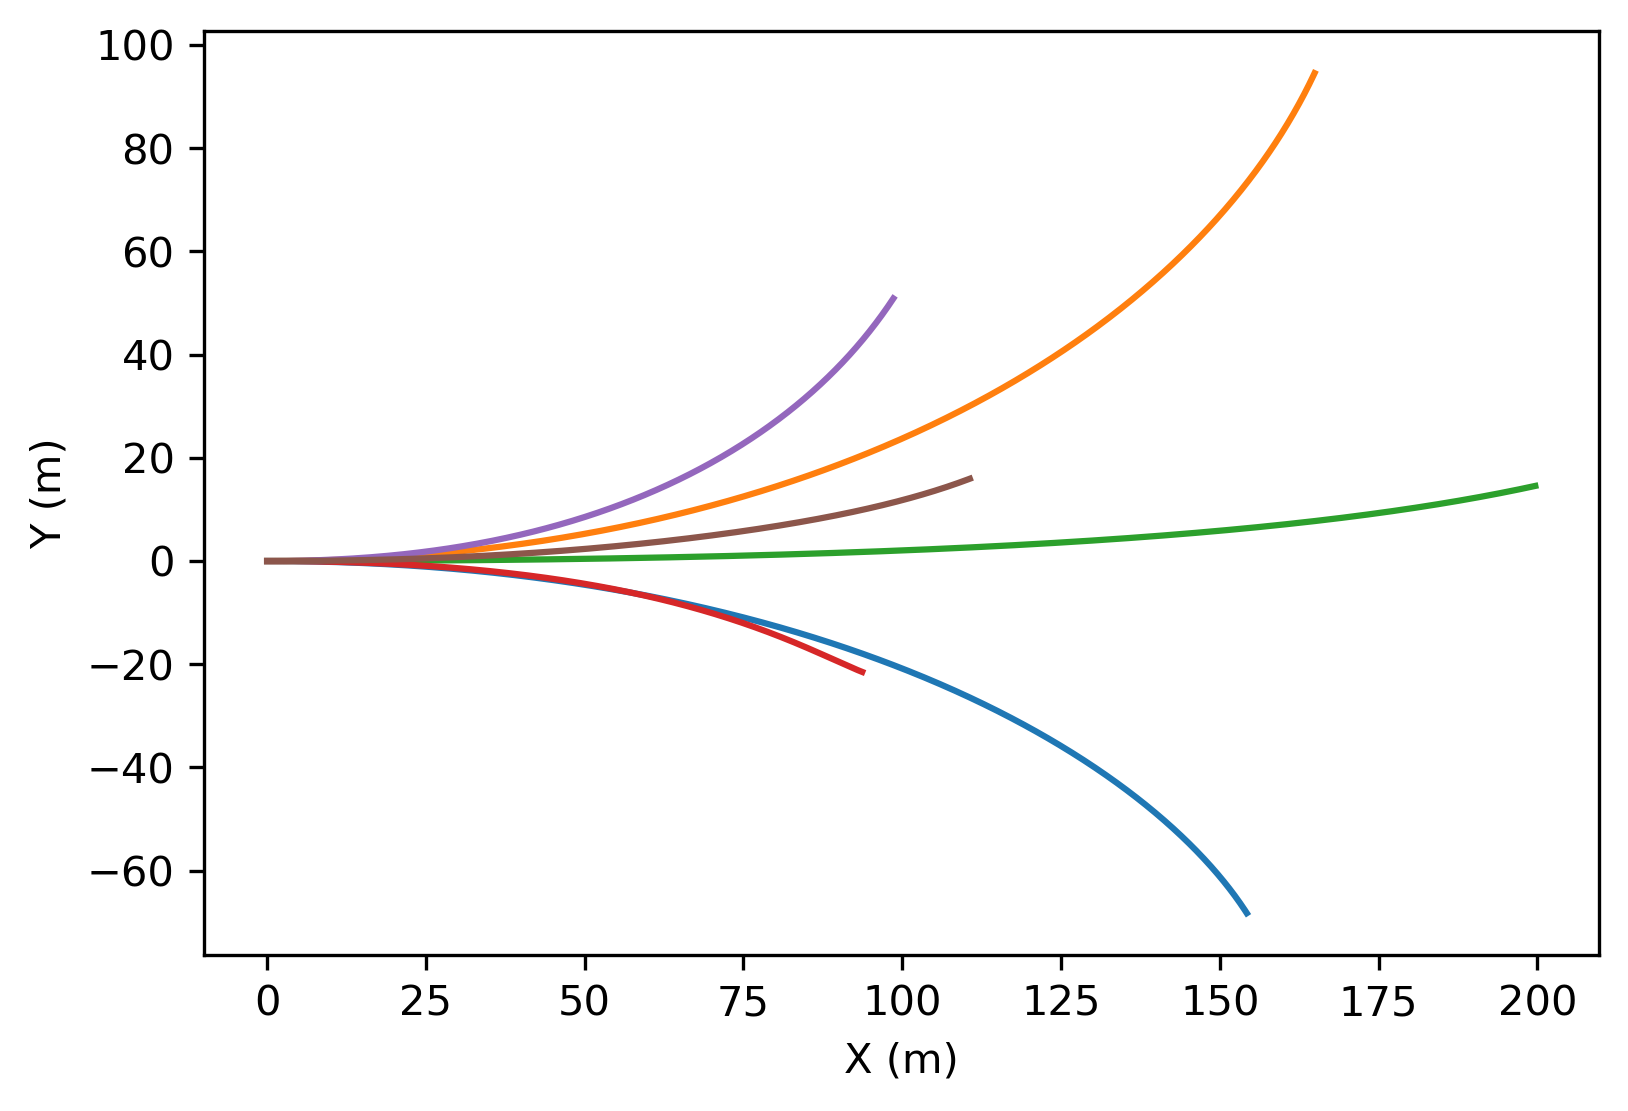
\includegraphics[width=\linewidth]{imagenes/golf_lateralXYcon.png}
    \caption{Caso con viento.}
    \label{fig:XYcom}
\end{subfigure}
\caption{Vista XY de la trayectoria de una pelota de golf.}
\label{fig:xygolf}
\end{figure}

\begin{figure}[H]
\centering
\begin{subfigure}[t]{0.49\textwidth}
    \centering
    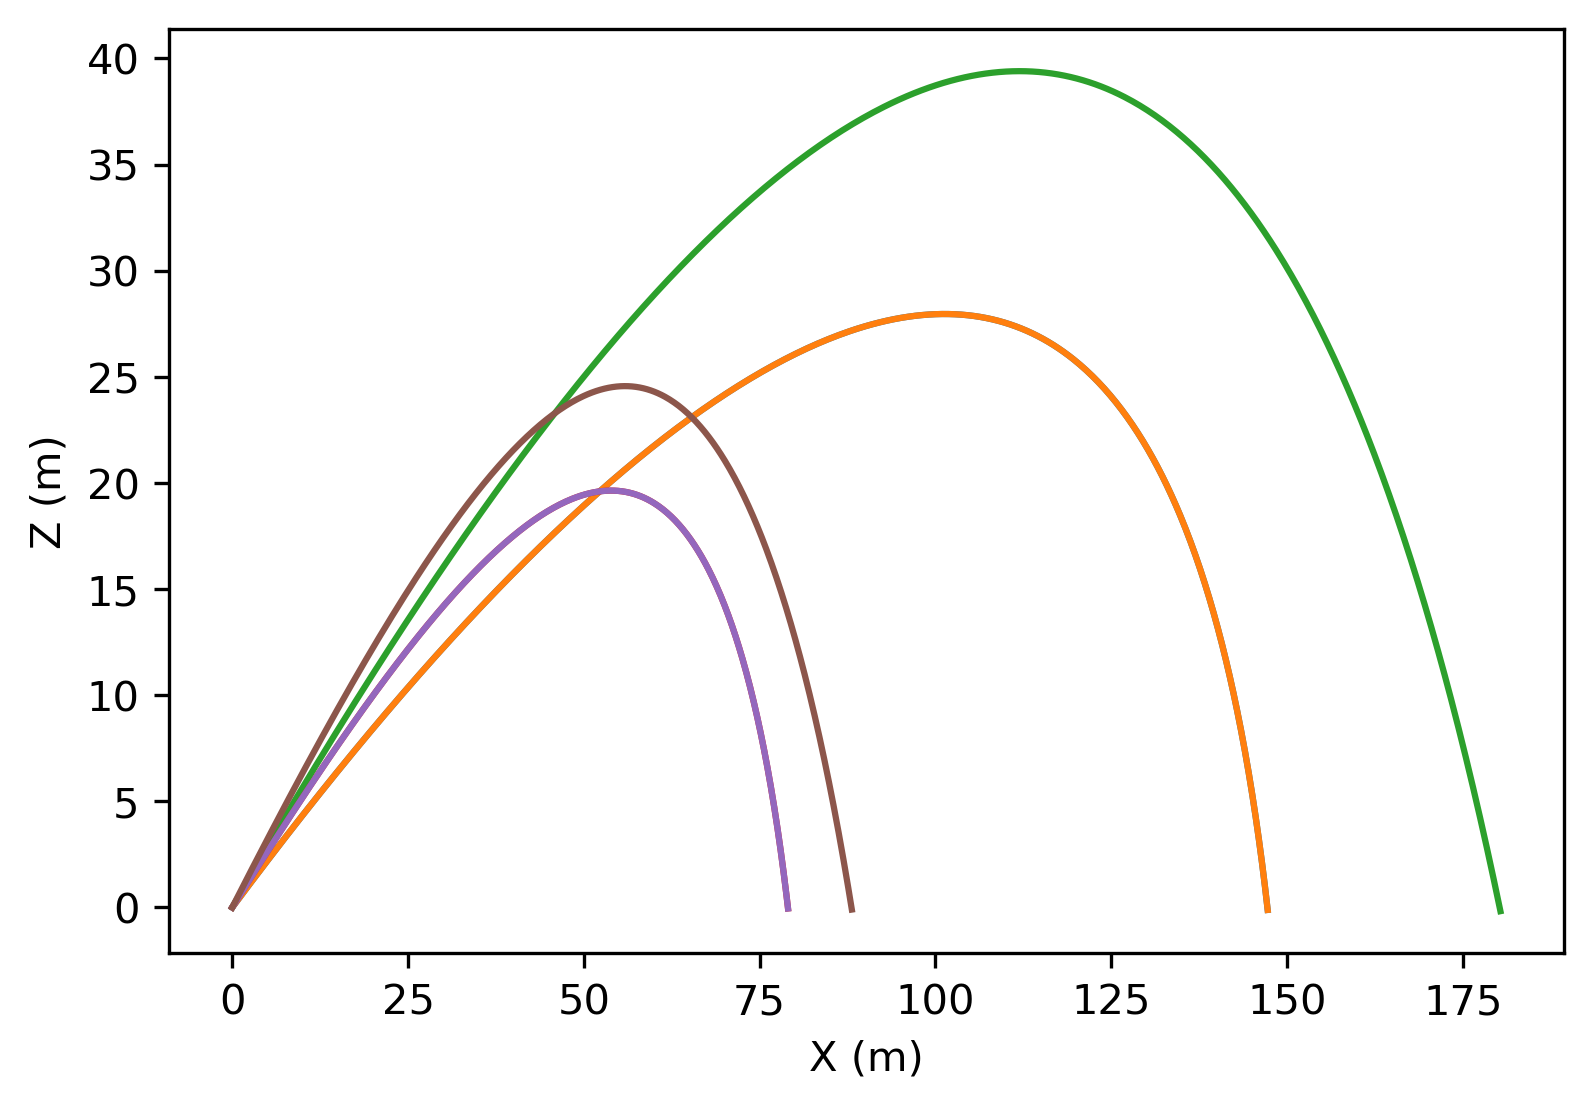
\includegraphics[width=\linewidth]{imagenes/golf_lateralXZsin.png}
    \caption{Caso sin viento.}
    \label{fig:XZsin}
\end{subfigure}
\hfill
\begin{subfigure}[t]{0.49\textwidth}
    \centering
    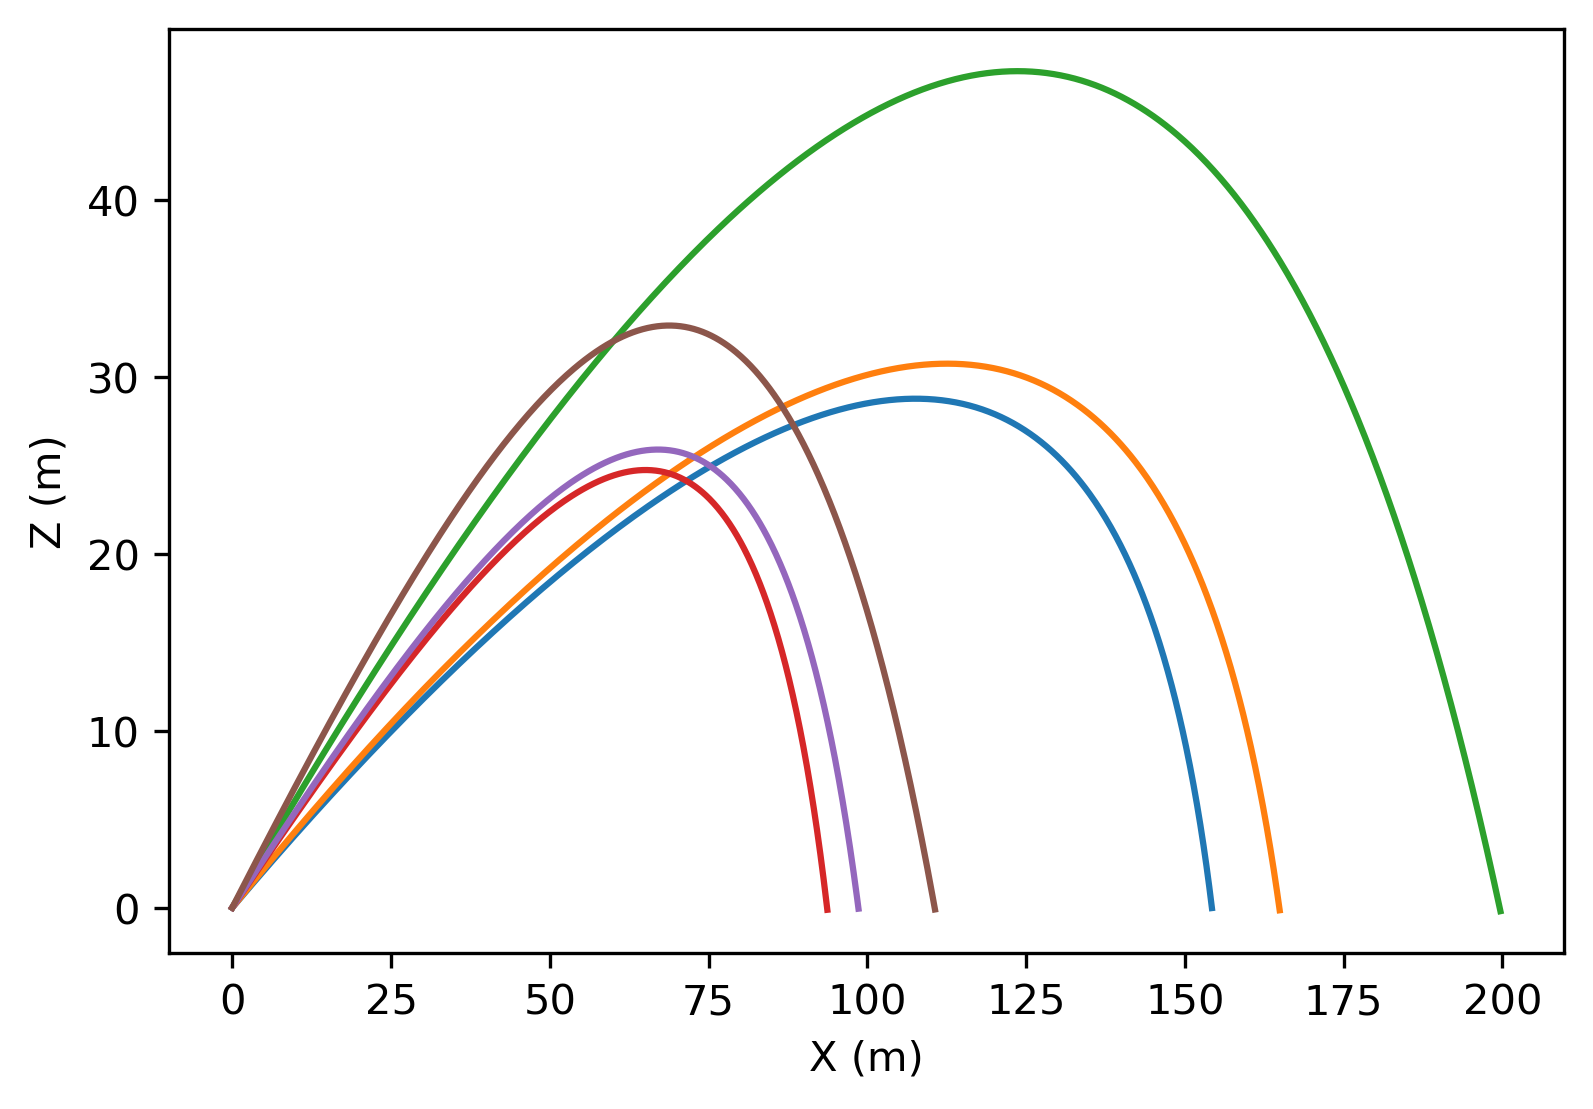
\includegraphics[width=\linewidth]{imagenes/golf_lateralXZcon.png}
    \caption{Caso con viento.}
    \label{fig:XZcom}
\end{subfigure}
\caption{Vista XZ de la trayectoria de una pelota de golf.}
\label{fig:xzgolf}
\end{figure}

\begin{figure}[H]
\centering
\begin{subfigure}[t]{0.49\textwidth}
    \centering
    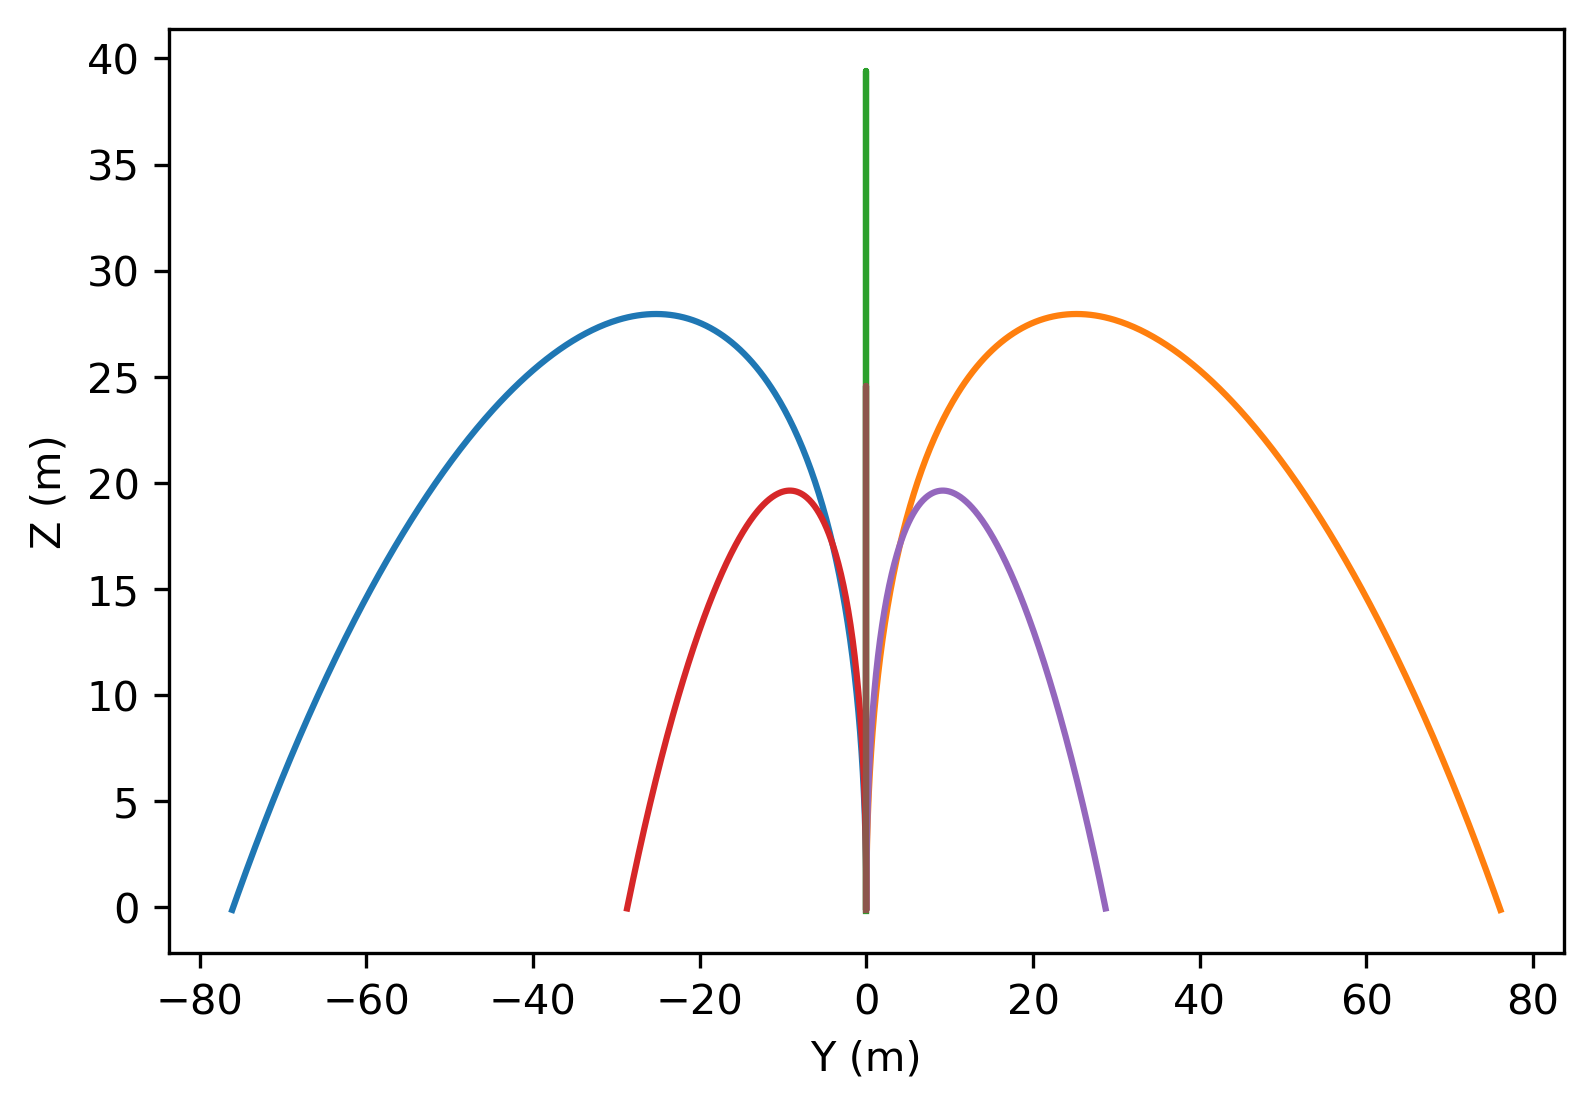
\includegraphics[width=\linewidth]{imagenes/golf_lateralYZsin.png}
    \caption{Caso sin viento.}
    \label{fig:YZsin}
\end{subfigure}
\hfill
\begin{subfigure}[t]{0.49\textwidth}
    \centering
    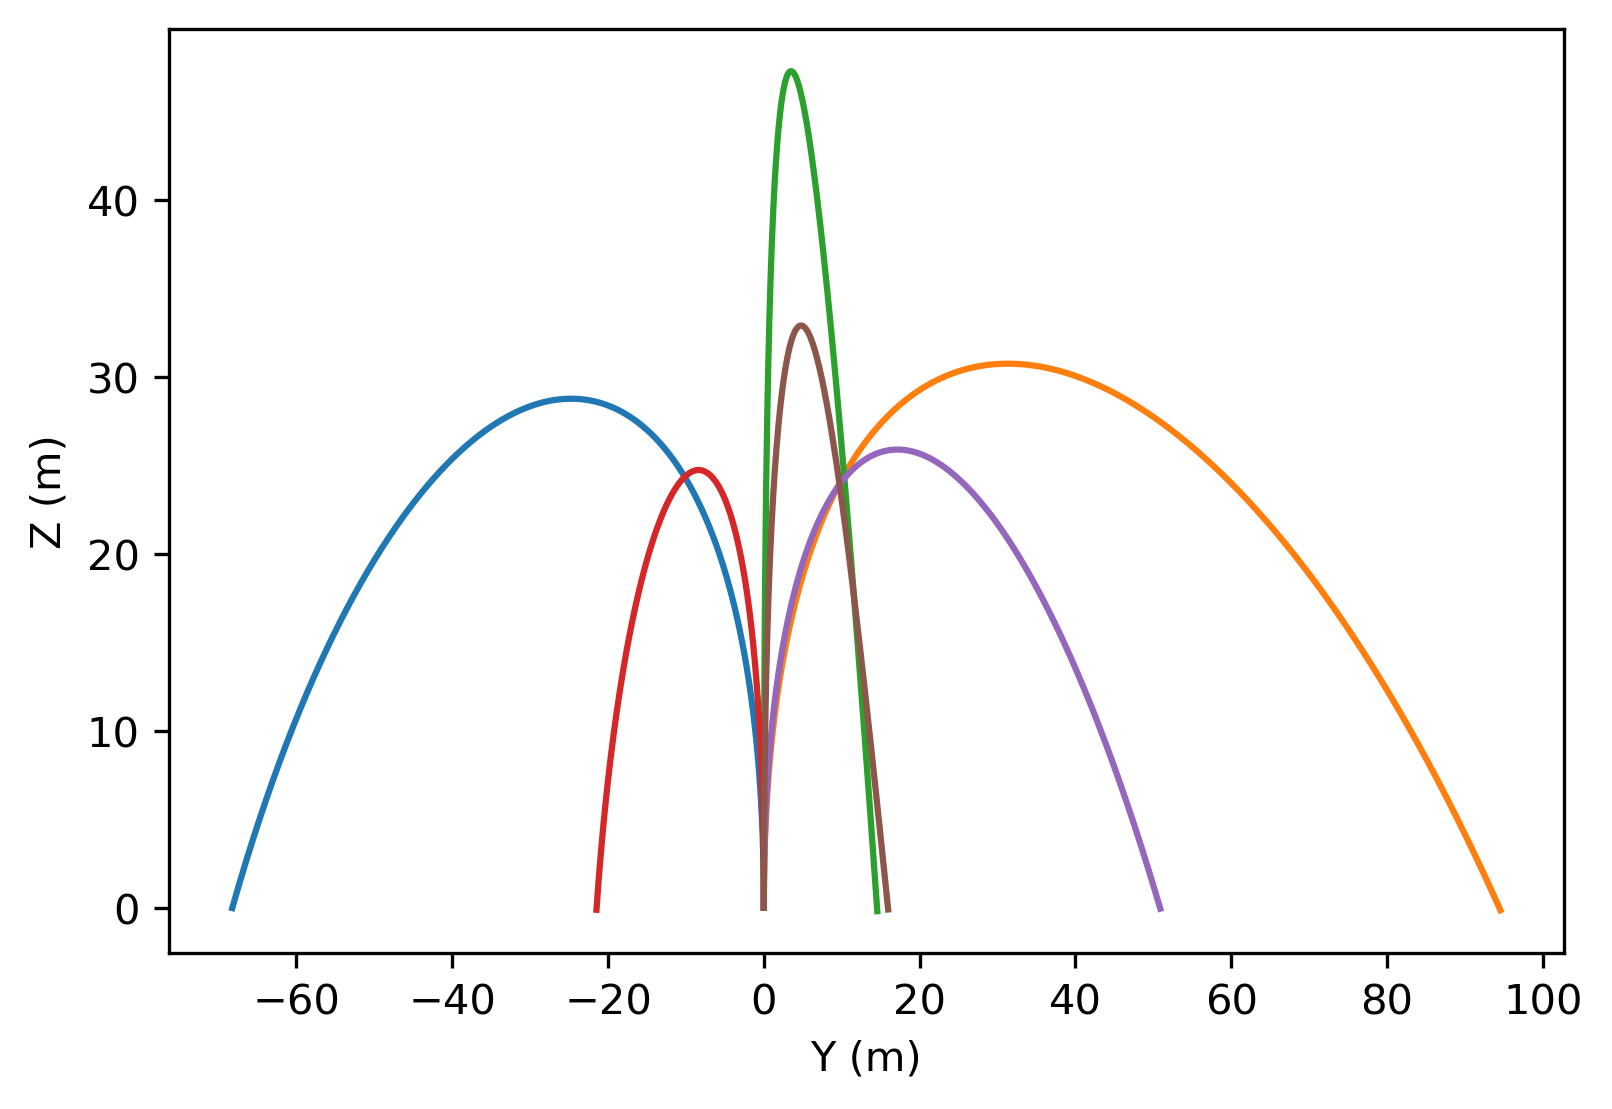
\includegraphics[width=\linewidth]{imagenes/golf_lateralYZcon.png}
    \caption{Caso con viento.}
    \label{fig:YZcom}
\end{subfigure}
\caption{Vista YZ de la trayectoria de una pelota de golf.}
\label{fig:yzgolf}
\end{figure}

\section{Discusión de resultados}

Los resultados obtenidos resaltan la importancia de la resistencia aerodinámica y de los efectos del viento y la rotación y su repercusión en la dinámica de los proyectiles reales.

En el caso del béisbol, el ángulo óptimo sin viento ($36^\circ$) es claramente inferior a los $45^\circ$ del modelo ideal parabólico sin rozamiento. Esto se debe a que la resistencia generada por el aire aumenta las pérdidas de energía durante el vuelo, que afecta especialmente a las trayectorias con gran componente vertical. La presencia del viento modifica tanto el alcance máximo como el ángulo óptimo, aumentando ambos si el viento va a favor (compensando parte del efecto de la resistencia del aire) y reduciendo ambos cuando el viento aumenta la velocidad relativa (viento en contra).

En el caso del golf, el comportamiento es aún más complejo debido a la dinámica tridimensional y al efecto Magnus. Para un ángulo fijo, la pelota rugosa alcanza distancias aproximadamente el doble que la lisa, lo cual confirma la importancia aerodinámica de las hendiduras (dimples). La reducción del coeficiente efectivo de arrastre en la pelota rugosa permite que el proyectil conserve velocidad durante más tiempo.

La inclusión del efecto Magnus genera desviaciones laterales significativas. En el caso optimizado sin viento, la desviación lateral alcanza hasta 76 m para la pelota rugosa, mientras que en la lisa es considerablemente menor. El efecto Magnus no solo introduce curvatura lateral sino que modifica también ligeramente el ángulo óptimo y el alcance máximo, reduciendo ambos.

Sin tener en cuenta el viento, el alcance máximo, el ángulo óptimo y la desviación lateral del lanzamiento tipo hook y tipo slice es igual. Esta simetría desaparece al considerar el caso con viento lo cual es visible tanto en los resultados numéricos como en cualquiera de las vistas de las trayectorias.

Finalmente, se hace evidente que la pelota rugosa llega hasta un alcance máximo mayor que la pelota lisa para cualquiera de los casos estudiados, resaltando también la importancia de la fuerza de arrastre al variar la rugosidad. Este efecto es fácilmente verificable, por ejemplo, con el caso de un lanzamiento hook con viento, donde una pelota rugosa puede llegar a 154.2 m de alcance mientras que una pelota lisa no podría pasar de 93.7 m. Esta amplificación del alcance es la razón por la cual se utilizan pelotas rugosas en el golf. No obstante, esto también funciona como argumento para pasar a utilizar pelotas lisas en vez de rugosas, ya que el tamaño de los campos sería reducible sin necesidad de reducir el número de golpes para terminar los hoyos.

\section{Conclusiones}

El estudio numérico del problema resalta la inadecuación del modelo parabólico para describir la dinámica de proyectiles reales y muestra la utilidad de la simulación numérica para problemas de dinámica no lineal. Además, la implementación de una resistencia aerodinámica reduce tanto el alcance como el ángulo óptimo del lanzamiento. Adicionalmente, el efecto Magnus introduce desviaciones laterales significativas que afectan a la trayectoria explicando el lanzamiento hook/slice. Por otro lado, el viento puede modificar notablemente la trayectoria de los proyectiles (alcance y ángulo óptimo) y romper la simetría del hook/slice que existiría sin viento. Finalmente, la rugosidad de la pelota se estudió en el caso del golf, explicando el uso de pelotas rugosas en vez de lisas para obtener golpes con alcances mayores. 

\begin{thebibliography}{9}

\bibitem{giordano}
N. J. Giordano and H. Nakanishi,
\textit{Computational Physics},
2nd ed., Pearson Prentice Hall, 2006.

\end{thebibliography}

\newpage
\appendix
\section*{Anexo A: Variables y condiciones iniciales empleadas}

\addcontentsline{toc}{section}{Anexo A: Variables y condiciones iniciales empleadas}

\subsection*{A.1 Variables físicas y dinámicas}

\begin{table}[H]
\centering
\begin{tabular}{ll}
\toprule
Símbolo & Significado físico \\
\midrule
$m$ & Masa del proyectil \\
$\vec{r}=(x,y,z)$ & Vector posición \\
$\vec{v}=(v_x,v_y,v_z)$ & Vector velocidad \\
$v$ & Módulo de la velocidad ($v=\sqrt{v_x^2+v_y^2+v_z^2}$) \\
$\vec{a}$ & Vector aceleración total \\
$\vec{g}$ & Aceleración gravitatoria \\
$g_{\text{eff}}$ & Gravedad corregida por altura \\
$R_T$ & Radio de la Tierra \\
$h$ & Altura sobre la superficie terrestre \\
$C_D$ & Coeficiente de arrastre \\
$\rho$ & Densidad del aire \\
$A$ & Área transversal del proyectil \\
$B_2$ & Parámetro efectivo de arrastre en béisbol \\
$v_d$ & Velocidad característica del modelo empírico \\
$\delta$ & Parámetro de transición del modelo empírico \\
$\vec{\omega}$ & Velocidad angular (espín) \\
$S_0$ & Constante asociada al efecto Magnus \\
$\vec{F}_D$ & Fuerza de arrastre \\
$\vec{F}_M$ & Fuerza de Magnus \\
$\Delta t$ & Paso temporal de integración \\
$\theta$ & Ángulo inicial de lanzamiento \\
\bottomrule
\end{tabular}
\caption{Variables empleadas en el desarrollo teórico y numérico.}
\end{table}

\subsection*{A.2 Condiciones iniciales — Simulación de béisbol}

Las condiciones iniciales generales empleadas en la simulación bidimensional de la pelota de béisbol fueron:

\begin{table}[H]
\centering
\begin{tabular}{ll}
\toprule
Parámetro & Valor utilizado \\
\midrule
$g$ & $9.81\,\text{m/s}^2$ \\
$R_T$ & $6.3 \times 10^6\,\text{m}$ \\
$\rho$ & $1.2\,\text{kg/m}^3$ \\
$v_0$ & $49\,\text{m/s}$ \\
$x_0$ & $0\,\text{m}$ \\
$y_0$ & $0\,\text{m}$ \\
$\Delta t$ & $0.01\,\text{s}$ \\
Barrido angular & $0^\circ \leq \theta \leq 90^\circ$ \\
Resolución angular & $0.1^\circ$ \\
Velocidad del viento & $v_{wx} = \pm \frac{49}{11}\,\text{m/s}, \quad v_{wy}=0$ \\
$v_d$ & $35\,\text{m/s}$ \\
$\delta$ & $5\,\text{m/s}$ \\
\bottomrule
\end{tabular}
\caption{Condiciones iniciales empleadas en la simulación de béisbol.}
\end{table}

\subsection*{A.3 Condiciones iniciales — Simulación de golf}

En el caso tridimensional de la pelota de golf las condiciones iniciales generales fueron:

\begin{table}[H]
\centering
\begin{tabular}{ll}
\toprule
Parámetro & Valor utilizado \\
\midrule
$g$ & $9.81\,\text{m/s}^2$ \\
$x_0,y_0,z_0$ & $0\,\text{m}$ \\
$v_0$ & $70\,\text{m/s}$\\
$\Delta t$ & $0.01\,\text{s}$ \\
Ángulos iniciales & Determinados mediante optimización \\
$m$ & $45.93 \times 10^{-3}\,\text{kg}$ \\
$R$ & $0.02135\,\text{m}$ \\
$A=\pi R^2$ & $1.43 \times 10^{-3}\,\text{m}^2$ \\
\bottomrule
\end{tabular}
\caption{Condiciones iniciales empleadas en la simulación de golf.}
\end{table}

\subsection*{A.4 Criterio de cálculo del alcance}

El alcance horizontal se estimó numéricamente mediante:

\[
\text{alcance} = \frac{x_{n}+x_{n-1}}{2}
\]

donde $x_n$ corresponde al primer punto con altura negativa y $x_{n-1}$ al último punto con altura positiva.\\
Paralelamente, la desviación lateral se estimó numéricamente mediante:

\[
\text{desviación lateral} = \frac{y_{n}+y_{n-1}}{2}
\]

donde $y_n$ corresponde al primer punto con altura negativa y $y_{n-1}$ al último punto con altura positiva.

\end{document}